%!TEX root = ../dissertation.tex
\begin{savequote}[75mm]
We must be prepared to accept the possibility that what we call ``the environment'' may lie, in part, within the skin of the biological organism
\qauthor{Herbert Simon (\citeyear{simon1955behavioral})}
\end{savequote}

% \chapter{Formalism}
\Chapter[Meta-level Markov decision processes]{Formalism}
% \begin{flushright}
% {\large\itshape Meta-level Markov decision processes}
% \vspace{1.3\baselineskip}
% \end{flushright}

\newthought{The key insight} underlying the proposed framework is that cognitive processes (including, for example, decision making) are themselves solutions to sequential decision problems. Drawing on a subfield of artificial intelligence known as \emph{rational metareasoning} \citep{matheson1968economic,russell1991principles}, we formalize this insight using the framework of \emph{meta-level Markov decision processes} (meta-level MDPs; \citealp{hay2012selecting}). In this framework, a cognitive process is formalized as a sequential process of executing computational actions that update an agent's beliefs about the world. At each moment, the agent must choose whether to continue deliberating, refining their beliefs but accruing computational cost, or to instead stop computing and make a decision. In the former case, they must additionally decide which computation to execute next (i.e., what to think about); in the latter case, they select the optimal action given their current belief and receive a reward associated with the external utility of that action.

In this chapter, I provide a formal description of the framework, identify technical challenges that arise when applying the framework, and discuss various strategies for addressing those strategies.

% We begin by introducing Markov decision processes (MDPs). Next, we define meta-level MDPs as extensions of standard MDPs. Finally, we define a specific meta-level MDP model for multi-attribute decision-making, which we will employ in our experimental case studies.

% Below, we give a high-level and intuitive overview of the general framework and its application to multi-attribute choice, the domain we will use in our case studies. A formal treatment is provided in Appendix~\ref{metamdp}.

% We begin by describing, in intuitive terms, how the framework can be applied to model multi-attribute decision-making. Next, we will formally define meta-level MDPs. Finally, we will return to the multi-attribute decision-making case, showing how the formalism can be applied to a specific case.

\begin{figure*}
  % \centering
  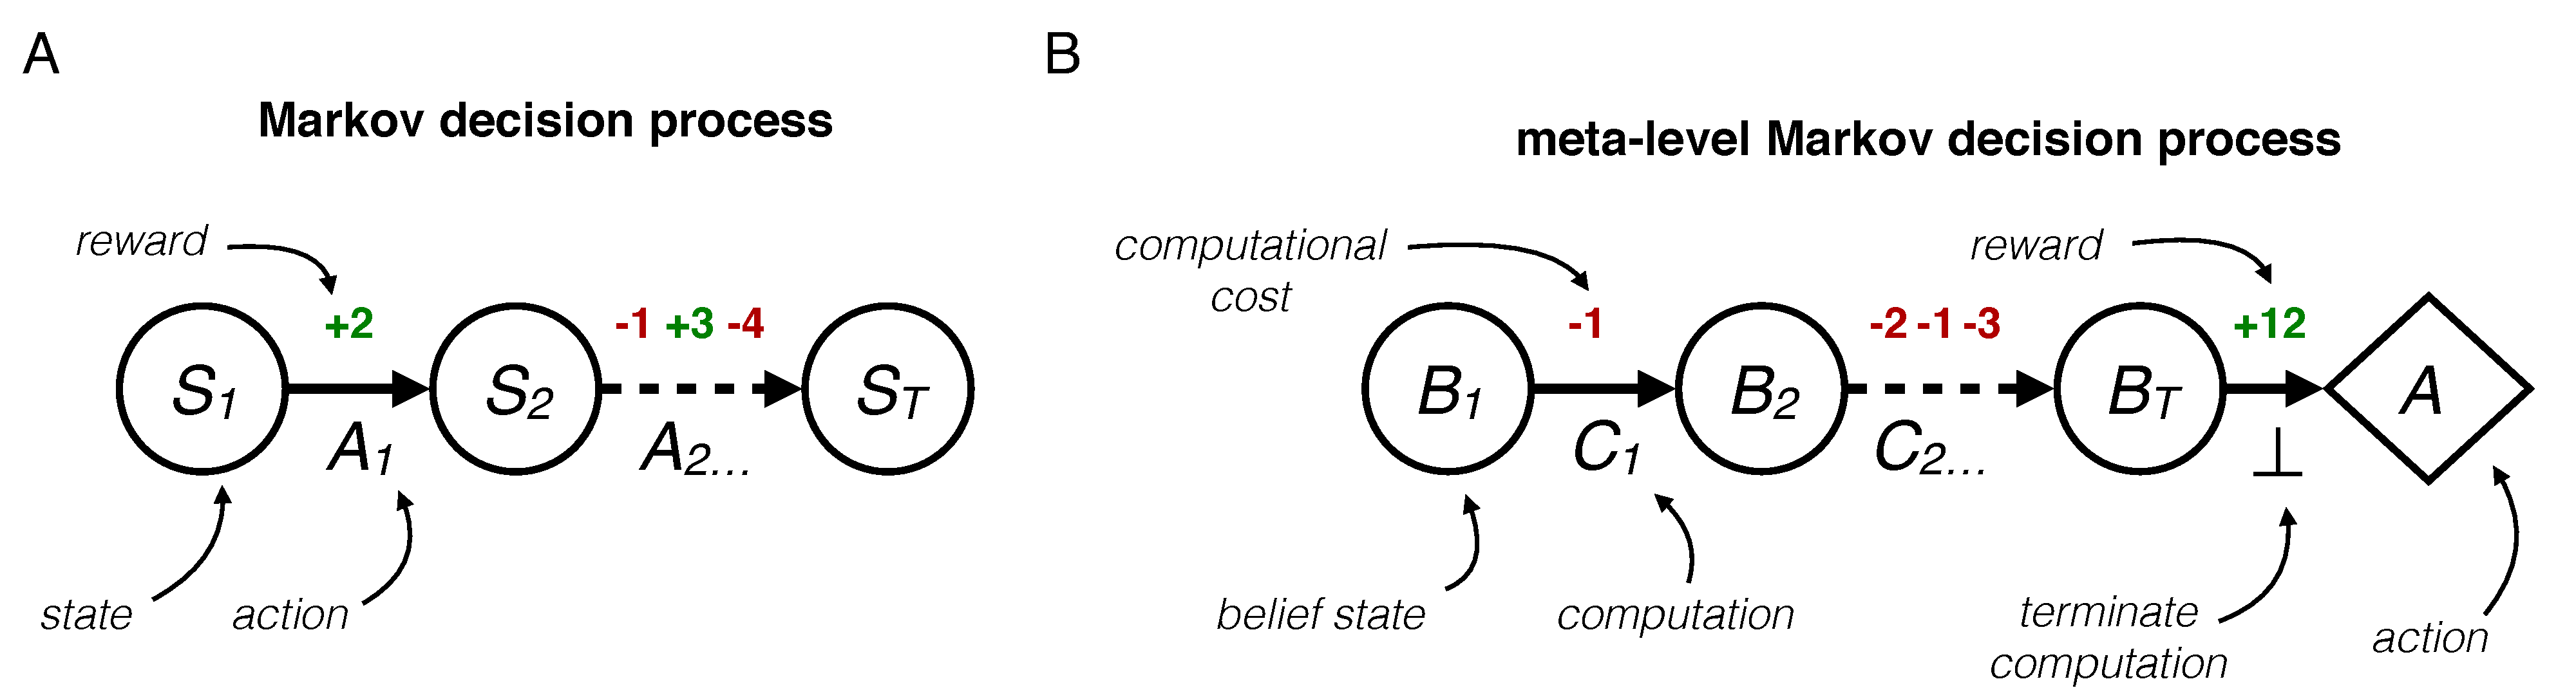
\includegraphics[width=\textwidth]{figs/metamdp.pdf}
  \caption{Formal framework: meta-level Markov decision processes.
  (A) A Markov decision process formalizes the problem of acting adaptively in a dynamic environment. The agent executes actions that change the state of the world and generate rewards, which the agent seeks to maximize.
  (B) A meta-level Markov decision process formalizes the problem of \emph{deciding how to act} when computational resources are limited. The agent executes computations that update their belief state and incur computational cost. When the agent executes the termination operation $\bot$, they take an external action based on their current belief state.}
  \label{fig:metamdp-diagram}
\end{figure*}


\section{Markov decision processes}

The core mathematical object underlying our approach is the Markov decision process (MDP), illustrated in Figure~\ref{fig:metamdp-diagram}A. MDPs are the standard formalism for modeling the sequential interaction between an agent and a stochastic environment. An MDP is defined by a set of states $\S$, a set of actions $\A$, a transition function $T$, and a reward function $r$. A state $s \in \S$ specifies the relevant state of the world. An action $a \in \A$ is an action the agent can perform. The transition function $T$ encodes the dynamics of the world as a distribution of possible future states for each possible previous state and action. Finally, the reward function $r$ specifies the reward or utility for executing a given action in a given state.

The standard goal in an MDP is to maximize the expected cumulative reward attained, that is, the \emph{return}. Importantly, this may require incurring immediate losses (negative rewards) in order to get to a state from which a highly rewarding action can be executed. It is typically assumed that the agent selects their actions based on the current state; the mapping from state to action is called a policy, denoted $\pi$. Solving an MDP amounts to finding a policy that maximizes the expected return, that is, a mapping from states to actions that, when followed, maximizes the total reward one will receive on average.

% An important property of MDPs is that there is at least one deterministic \emph{optimal policy}; that is, there is a mapping from states to actions that, when followed, will produce the maximum possible return. 

In addition to their foundational role in artificial intelligence \citep{sutton2018reinforcement}, MDPs are widely used in models of human decision-making \citep{dayan2008decision}. MDPs are the formal foundation for models of reinforcement learning \citep{niv2009reinforcement} and model-based planning \citep{huys2015interplay,botvinick2012planning}, as well as competition between the two systems \citep{daw2005uncertaintybased,keramati2011speed,kool2017costbenefit}. They have also been used to study information-seeking \citep{gottlieb2013informationseeking,hunt2016approachinduced}, generalization \citep{tomov2021multitask}, and hierarchical abstraction \citep{solway2014optimal,botvinick2009hierarchically}. However, with a few notable exceptions \citep{dayan2008serotonin,drugowitsch2012cost,tajima2016optimal}, MDPs have primarily been used to model the sequential decision problems posed by the external world. In the following section, we show how this framework can be applied to model the sequential decision problem posed by one's own cognitive architecture.

\section{Meta-level Markov decision processes}

% The concept is thus very similar to \emph{elementary information processes} \citep{chase1978elementary,simon1979information,posner1982information,payne1988adaptive}. 

Meta-level Markov decision processes (meta-level MDPs) extend the standard MDP formalism to model the sequential decision problem posed by resource-bounded computation \citep{hay2012selecting}. Like a standard MDP, there is a set of states $\S$, a set of actions $\A$, and a reward function $r\object$ (we omit the transition function because we focus on one-shot decisions). These define the \emph{object-level} problem: the external problem the agent must solve in the world. Additionally, the meta-level MDP defines a set of beliefs $\B$, a set of computations $\C$, and meta-level transition and reward functions, $T\meta$ and $r\meta$. These define the \emph{meta-level} problem: how to allocate limited computational resources in the service of solving the object-level problem.

As illustrated in Figure~\ref{fig:metamdp-diagram}B, the meta-level problem is itself a sequential decision problem, analogous to one defined by a standard MDP. However, in the meta-level problem, the states are replaced by beliefs (mental states) and the actions are replaced by computations (cognitive operations). The meta-level transition function describes how computations update beliefs, and the meta-level reward function captures both computational cost and the object-level reward of the action that is ultimately executed. We provide a formal definition below.

We define a meta-level MDP as $(\S, \A, r\object, \B, \C, T\meta, r\meta)$. The first three components define the object-level problem. They have the same interpretation as $\S$, $\A$, and $r$ in a standard MDP. Note that we omit the transition function because we limit our attention to problems in which all computation must be performed before any actions are taken.\footnote{%
  Sequential object-level problems can be accomodated by letting each element of $\A$ be a sequence of actions. In such cases, the object-level transition function will be implicitly embedded in $r\object$. Forcing all computation to occur before any action is taken does not result in a loss of performance when the object-level transition function is deterministic. See Chapter~\ref{sec:planning} for an application to deterministic sequential problems.
} The latter four components define the meta-level problem. We now define each of the seven components in turn.

\paragraph{States}
A state $s \in \S$ captures the relavent state of the world.

\paragraph{Beliefs}
A belief state $b \in \B$ captures the agent's current knowledge about the relevant state of the world. Formally, a belief is a distribution states, $\B \subseteq \Delta(\S)$. Note that $\Delta(\S)$ denotes the set of all possible distributions over $\S$.
% One typically makes distributional assumptions that restrict the space of beliefs the agent can entertain, such that $\B \subset \Delta(\S)$. 
Importantly, contrary to a standard rational treatment of beliefs, the belief states in a meta-level MDP do not include all the information that is available to the DM. Instead, the belief state only contains information that is immediately accessible, excluding, for example, long-term memories and the number of calories in every box of cereal on a shelf.

\paragraph{Computations}
A computational operation $c \in \C$ is a primitive operation afforded by the computational architecture. Formally, it is a meta-level action that updates the belief in much the same way as a regular action changes state. All meta-level MDPs include the termination operation $\bot$, which denotes that computation should be terminated and an action should be selected based on the current belief state. We further explain belief updating and termination in the following two paragraphs.

\paragraph{Transition function}
The meta-level transition function $T\meta: \B \times \C \times \S \rightarrow \Delta(\B)$ describes how computation updates beliefs. At each time step, the next belief is sampled from a distribution that depends on the current belief, the computational operation that was just executed, and the true state of the world, that is,
\begin{equation}
b_{t+1} \sim T\meta(b_t, c_t, s).
\end{equation}
The transition function thus defines the core structure of the computational architecture. Following previous work \citep{matheson1968economic,hay2012selecting}, we assume that the effect of computation is to generate or reveal information about the true state of the world, which is then integrated into the belief state. Thus, in expectation, computation has the effect of making one's beliefs more precise and accurate, although an individual computation may yield misleading information. 

% This formalization is quite natural for many types of cognitive operations, such as memory recall and mental simulation. However, it can also be applied in less obvious cases; for example, performing an addition operation generates previously inaccessible information about the value of the sum of two numbers.

% the marginalized meta-level transition function is always stochastic. Without knowledge of the true object-level state $s$, the DM cannot predict exactly how a computation will change her belief---if she could, she could simply adopt that updated belief without performing the computation. 

\paragraph{Reward function}
The meta-level reward function $r\meta: \B \times \C \times \S \rightarrow \R$ describes both the costs and benefits of computation. For the former, $r\meta$ assigns a strictly negative reward for all non-terminating computational operations,
%
\begin{equation}
r\meta(b, c, s) = -\cost(c) \text{ for } c \neq \bot.
\end{equation}
%
The cost of computation may include multiple factors, such as energetic costs and opportunity costs. 

Intuitively, the benefit of computation is that it allows one to make better decisions. This is captured by the meta-level reward for the termination operation $\bot$, defined as the true utility of the external action that the DM would execute given the current belief. We assume that the action is selected optimally. Thus,
%
\begin{equation}\label{eq:term-reward}
r\meta(b, \bot, s) = r\object(s, a^*(b)).
\end{equation}
%
where
%
\begin{equation}\label{eq:object-action}
a^*(b) = \argmax_a \expect{r\object(s, a)}{s \sim b}
\end{equation}
%
In English, the meta-level reward for termination is the \emph{true} utility of the action\footnotemark{} with maximal \emph{estimated} utility.

\footnotetext{
  For notational clarity, we have assumed a single optimal action. When multiple actions have the same expected value, we assume that ties are broken randomly; thus, $a^*(b)$ is more precisely a uniform distribution over all optimal actions, and $r\meta(b, \bot, s)$ takes an expectation over them.
}

\paragraph{Policy}\label{sec:metamdp-policy}

The solution to a meta-level MDP takes the form of a policy $\pi: \B \rightarrow \Delta(\C)$ that (perhaps stochastically) selects which computation to perform in each possible belief state. The optimal policy is the one that maximizes expected meta-level return,
%
\begin{equation}\label{eq:optimal-policy}
  \pi^* = \argmax_\pi \expect{
    \sum_{t=1}^T r\meta(B_t, C_t, S)
  }{
    C_t \sim \pi
  }.
\end{equation}


\subsection{Value of computation}

This suggests a strategy for selecting computations optimally. For each item, estimate how much one's decision would improve if one sampled from it (and then continued sampling optimally). Subtract from this number the cost of taking the sample (and also the estimated cost of the future samples). Now identify the item for which this value is maximal. If it is positive, it is optimal to take another sample for this item; otherwise, it is optimal to stop sampling and make a decision.

This basic logic is formalized in rational metareasoning as the \textit{value of computation} (VOC; \citealp{russell1991principles}). Formally, $\VOC(b, c)$ is defined as the expected increase in total metalevel reward if one executes a single computation, $c$, and continues optimally rather than making a choice immediately (i.e., executing $\bot$):
$$
\VOC(b_t, c) = R(b_t, c) + \E \left[
  \sum_{t'=t+1}^T R(b_{t'}, c_{t'})\ \Big\vert\ c_{t'} \sim \pi^*(b_{t'}) 
\right] - R(b, \bot).
$$

We can then define the optimal policy as selecting computations with maximal VOC:
$$
\pi^*(b) \sim \text{Uniform}(\argmax{c} \VOC(b, c)).
$$
For those familiar with reinforcement learning, this recursive joint definition of $\pi^*$ and VOC is exactly analogous to the joint definition of the optimal policy with the state-action value function, $Q$ \citep{sutton2018reinforcement}. Indeed, $\VOC(b, c) = Q(b, c) - R(b, \bot)$. 

\subsection{Optimal metalevel policy}

\todo{shorten, maybe move some material to metamdp section}

The solution to a metalevel MDP takes the form of a Markov policy, $\pi$, that stochastically selects which computation to take next given the current belief state. Formally, $c_t \sim \pi(b_t)$. The optimal metalevel policy, $\pi^*$, is the one that maximizes expected total metalevel reward,
\begin{equation*}
  \pi^* = \argmax{\pi} \E \left[ \sum_t^T R(b_t, c_t) \ \Big\vert\ c_t \sim \pi(b_t) \right].
\end{equation*}
Replacing $R$ with its definition, we see that this requires striking a balance between the expected value of the chosen item and the computational cost of the samples that informed the choice,
\begin{equation*}
  \pi^* = \argmax{\pi} \E \left[
     \max_i \mu_T^{(i)} - \sum_t^{T-1} \cost(b_t, c_t)
   \ \Big\vert\ c_t \sim \pi(b_t) \right].
\end{equation*}
That is, one wishes to acquire accurate beliefs that support selecting a high-value item, while at the same time minimizing the cost of the samples necessary to attain those beliefs. This suggests a strategy for selecting computations optimally. For each item, estimate how much one's decision would improve if one sampled from it (and then continued sampling optimally). Subtract from this number the cost of taking the sample (and also the estimated cost of the future samples). Now identify the item for which this value is maximal. If it is positive, it is optimal to take another sample for this item; otherwise, it is optimal to stop sampling and make a decision.

This basic logic is formalized in rational metareasoning as the \textit{value of computation} (VOC; \citealp{russell1991principles}). Formally, $\VOC(b, c)$ is defined as the expected increase in total metalevel reward if one executes a single computation, $c$, and continues optimally rather than making a choice immediately (i.e., executing $\bot$):
$$
\VOC(b_t, c) = R(b_t, c) + \E \left[
  \sum_{t'=t+1}^T R(b_{t'}, c_{t'})\ \Big\vert\ c_{t'} \sim \pi^*(b_{t'}) 
\right] - R(b, \bot).
$$
In our model, this can be rewritten
$$
\VOC(b_t, c) = -\cost(b_t, c) + \E \left[ 
  \max_i \mu_T^{(i)} - \sum_{t'=t+1}^{T-1} \cost(b_{t'}, c_{t'})
  \Big\vert\ c_{t'} \sim \pi^*(b_{t'})
\right] -  \max_i \mu_t^{(i)}.
$$
That is, the VOC for sampling a given item in some belief state is the expected improvement in the value of the chosen item (rather than making a choice based on the current belief) minus the cost of sampling that item and the expected cost of all future samples.

We can then define the optimal policy as selecting computations with maximal VOC:
$$
\pi^*(b) \sim \text{Uniform}(\argmax{c} \VOC(b, c)).
$$
For those familiar with reinforcement learning, this recursive joint definition of $\pi^*$ and VOC is exactly analogous to the joint definition of the optimal policy with the state-action value function, $Q$ \citep{sutton2018reinforcement}. Indeed, $\VOC(b, c) = Q(b, c) - R(b, \bot)$. 

Finally, by definition, $\VOC(b,\bot)=0$ for all $b$. Thus, the optimal policy terminates sampling when no computation has a positive VOC.

\subsection{Bayesian metalevel policy search}\label{sec:BMPS}

This method is based on an approximation of the VOC as a linear combination of features,
\begin{equation}\label{eq:vochat}
  \begin{aligned}
    \VOCapprox =& w_{1}\VOImy(b,c)+w_{2}\VPIitem(b,c) +
     w_{3}\VPI(b) -(\cost(c)+w_{4}),
  \end{aligned}
\end{equation}
for all $c\neq\bot$, with $\widehat{\VOC}(b, \bot; \vec{w}) = \VOC(b,\bot)=0$.

We briefly define the features here, and provide full derivations in Appendix~\ref{app:attention-derivations}. The VOI terms quantify the \textit{value of information} \citep{howard1966information} that might be gained by different additional computations. Note that the VOI is different from the VOC because the latter includes the costs of computation as well as its benefits. In general, the VOI is defined as the expected improvement in the utility of the action selected based on additional information rather than the current belief state: $E_{\tilde{b} \mid b}[R(\tilde{b}, \bot) - R(b, \bot)]$, where $\tilde{b}$ is a hypothetical future belief in which the information has been gained, the distribution of which depends on the current belief.

$\VOImy(b,c)$ denotes the expected improvement in choice utility from drawing one additional sample from item $c$ before making a choice, as opposed to making a choice immediately based on the current belief, $b$. $\VPIitem(b,c)$ denotes the expected improvement from learning the true value of item $c$, and then choosing the best item based on that information. Finally, $\VPI(b)$ denotes the improvement from learning the true value of \text{every} item and then making an optimal choice based on that complete information.

Together, these three features approximate the expected value of information that could be gained by the (unknown) sequence of future samples. Importantly, this true value of information always lies between the lower bound of $\VOImy$ and the upper bound of $\VPI$ (see \Fig{fig:attention-voi}), implying that the true VOI is a convex combination of these two terms. Note, however, that the weights on this combination are not constant across beliefs, as assumed in our approximation. Thus, including the $\VPIitem$ term, improves the accuracy of the approximation, by providing an intermediate value between the two extremes. Finally, the last two terms in Equation~\ref{eq:vochat} approximate the cost of computation: $\text{cost}(c)$ is the cost of carrying out computation $c$ and $w_{4}$ approximates the expected future costs incurred under the optimal policy.

Although maximizing $\VOCapprox$ identifies the policy with the best performance, it is unlikely that humans make attentional decisions using such perfect and noiseless maximization. Thus, 
we assume that computations are chosen using a Boltzmann (softmax) distribution   \citep{mcfadden2001economic} given  by
\[
\pi(c \mid b; \mathbf{w}, \beta) \propto \exp \left\{ \beta\VOCapprox \right\},
\]
where the inverse temperature, $\beta$, is a free parameter that controls the degree of noise. Note that computation selection is fully random when $\beta=0$ and becomes deterministic as $\beta\rightarrow\infty$.



To identify the weights used in the approximation, we first assume that $w_{i}\ge0$ and $w_{1}+w_{2}+w_{3}=1$, since $w_{1:3}$ features form a convex combination and $w_4$ captures the non-negative future cost.